\documentclass[9pt,twocolumn,twoside]{../../styles/osajnl}
\usepackage{fancyvrb}
\journal{i524}
\title{Google BigQuery - A data warehouse for large-scale data analytics}

\author[1]{Sagar Vora}

\affil[1]{School of Informatics and Computing, Bloomington, IN 47408, U.S.A.}

\dates{\today}

\ociscodes{BigQuery, BigData, Google, Cloud, Database, IaaS, PaaS, SaaS, SQL}

% replace this with your url in github/gitlab
\doi{\url{https://github.com/cloudmesh/sp17-i524/raw/master/paper2/S17-IR-2041/report.pdf}}


\begin{abstract}

The amount of relational data generated is increasing rapidly since it
is generated through a large number of sources. Moreover this data is
the information which companies like to explore and analyse quickly to
identify solutions to business. Therefore, the need to solve the
problem of traditional database management systems in order to support
large volumes of data arises Google's BigQuery platform. Google
BigQuery is an enterprise data warehouse used for large scale data
analytics. A user can store and query the massive datasets by storing
data in BigQuery and quering the database. BigQuery runs in cloud
using the processing power provided by Google's infrastructure and
provides SQL-like queries to perform analysis on masssive quantities
of data, providing real-time insights about the data.\newline
\end{abstract}

% \setboolean{displaycopyright}{true}

\begin{document}

\maketitle

\section{Introduction}
Nowadays, the amount of data being collected, stored and processed
continues to grow rapidly. Querying this massive datasets can be time
consuming and expensive without the right hardware and
infrastructure. BigQuery\cite{www-bigquery} solves this problem by
providing super-fast, SQL-like queries, using the processing power of
Google's infrastructure. Google BigQuery\cite{bigquery-paper} is a
cloud web service data warehouse used for large-scale data
processing. It is suitable for businesses that cannot afford to spend
a huge amount of investment in infrastructure to process a huge amount
of information. This platform allows to store and retrieve large
amounts of information in near real time as well as providing some
important analysis of the data which is stored.

\section{Google BigQuery}
To solve the architectural problems faced by
Hadoop\cite{www-apache-hadoop} MapReduce\cite{mapreduce-article},
Google developed Dremel\cite{dremel-paper} application in order to
process large volumes of data. Dremel was designed to deliver high
performance on data which was spread across a huge range of multiple
servers and SQL support. But in 2012 at Google I/O event, it was
announced that they would no longer support Dremel and this led to the
beginning of BigQuery which became then the high-performance cloud
offering of google. BigQuery makes use of SSL (Secure Sockets Layer)
to take care of the security concerns related to cloud management.

\subsection{System Architecture and Internal Structure}

Google BigQuery platform is a Software As a Solution (SaaS) model in
the cloud. As seen in figure \ref{fig:architecture} data which is
generated from a variety of sources like event logs, relational
databases, IoT devices like sensors, actuators, social media websites,
Informatica\cite{www-informatica} applications, etc is loaded in the
databases which are created in BigQuery.

\begin{figure}[htbp]
\centering
\fbox{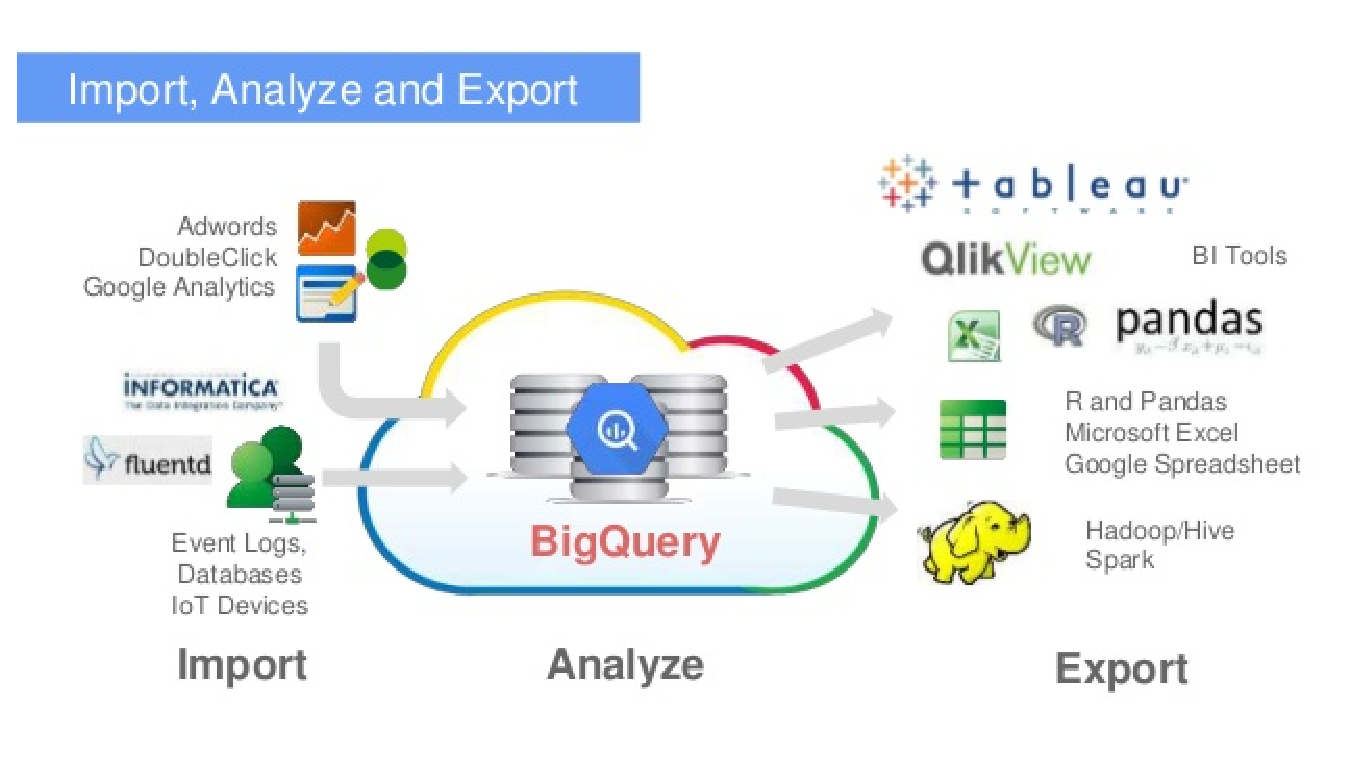
\includegraphics[width=\linewidth]{images/architecture}}
\caption{\cite{www-bigquery-slideshare} System Architecture of
  BigQuery}
\label{fig:architecture}
\end{figure}

\noindent
This data can then be processed and anaylsed using some algorthmic
logic or applying some processing tool. Finally the data can then be
represented and exported using Tableau\cite{www-tableau},
Qlikview\cite{www-qlik}, MS Excel\cite{www-excel} and other BI
tools. It can also be exported on Hadoop system for parallel
processing.\newline Now to store data in BigQuery, you need to create
Projects. Projects\cite{www-bigquery-documentation} in BigQuery act as
top-level containers which store the BigQuery data. Each project is
referenced by a name and unique ID. Tables in BigQuery store the
actual data where each table has a schema which describes the field
name, types and other information. In BigQuery each table must belong
to a dataset.Datasets help to organise the tables and control the
access to it.

\noindent

\section{Features of BigQuery}
Google BigQuery presents some characteristics like velocity,
simplicity, and multiple access methods.

\subsection{Velocity}

BigQuery can process millions of information in seconds because of its
columnar storage, and tree-like architecture.

\subsection{Columnar Storage and Tree Architecture}
The data instead of being stored in terms of rows like in standard
SQL, is stored as columns and thus storage is oriented as shown in
figure \ref{fig:rowvscolumnarstorage}. This not only results in fast
access to data but also results in scanning only the required values,
which largely reduces latency. This also results in a higher
compression ratios. Google reports\cite{www-rowvscolumnstorage} that
``BigQuery can achieve columnar compression ratios of 1:10 as opposed
to 1:3 when storing data in a traditional row-based format''.

\begin{figure}[htbp]
\centering
\fbox{\includegraphics[width=\linewidth]{images/rowvscolumnstorage}}
\caption{\cite{www-rowvscolumnstorage} Row-oriented vs Column-oriented
  Storage in tree architecture}
\label{fig:rowvscolumnarstorage}
\end{figure}

\noindent
Moreover the tree-like architecture is used for processing queries and
aggregating results across variety of different nodes. The tree-like
structure also helps in retrieving data faster. \newline Let us see
this with the help of 2 examples.

\noindent
Considering the column-oriented storage in tree architecture format in
the figure \ref{fig:rowvscolumnarstorage}, lets refer node A as our
root server, node B being an intermediate server and C, D, E being
leaf servers having local disk storage space.\newline

\noindent
Example 1: Fast-retrieval \newline Statement: Find out all the
customer names whose name starts with ‘A’.\newline
\noindent
Assuming node C contains customer names.  Hence, it is as simple as
traversing A -> B -> C and looking at the datasets Cr1 and Cr2 for
names starting with 'A'. One need not look at the paths from A -> B ->
D and A -> E. Hence, in this simple scenario, A query may not scan the
entire storage structure of the BigQuery and hence speeds up
retrieving the information. Here the reason why the query looks only
in the path A -> B -> C because BigQuery knows that all the customer
names starting with A have been placed in the local disk storage at
node C itself. \newline

\noindent
Example 2: Parallel Processing \newline Statement: Count all the
customer whose names starting with ‘A’. \newline

\begin{enumerate}[noitemsep,topsep=0pt]
\item Root node A sends out the query to node B which in turn
  translates the query to sum the names of all the customers starting
  with ‘A’. \item Now after translating, node B passes this query to
  leaf node C which has data stored in columnar format in the form of
  r1 and r2 tables. \item node C accesses these tablets in parallel,
  and counts the number of customers whose names start with ‘A’ and
  passes the count of Cr1 and Cr2 to node B which sums the result and
  passes it to the root Aas the output of the query. \end{enumerate}

\noindent
So this not only increases the speed of retriving the information but
also the goal of parallel processing which is the need in quering huge
datasets is also achieved.

\subsection{Simplicity}
Figure \ref{fig:bigqueryinterface} shows the simple user interface
provided by BigQuery. The dataset stored in BigQuery can be easily
queried using SQL-like queries.

\begin{figure}[htbp]
\centering
\fbox{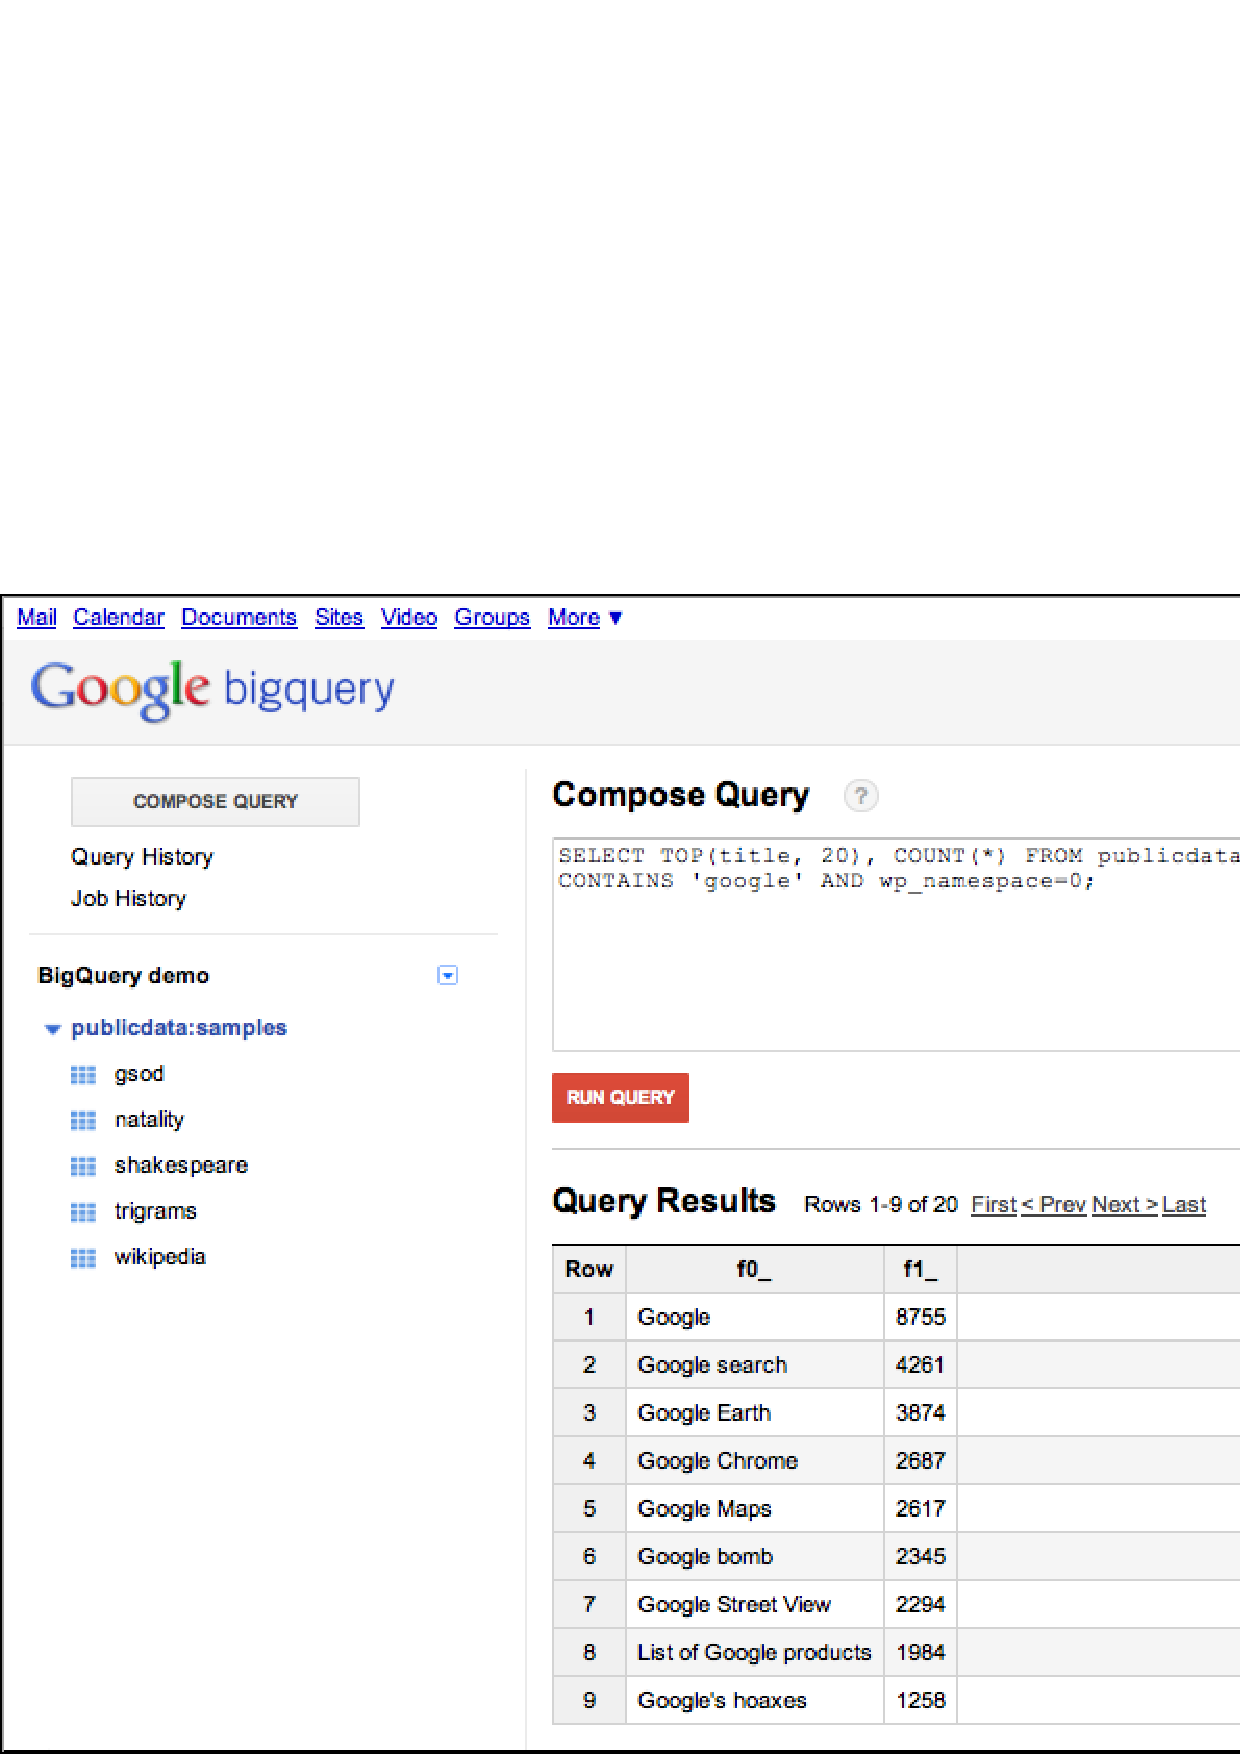
\includegraphics[width=\linewidth]{images/userinterface}}
\caption{\cite{www-userinterface-bigquery} Big Query Sample User
  Interface}
\label{fig:bigqueryinterface}
\end{figure}

\noindent
You can enter your query in the text area provided and the results
will be displayed below. At the left side of the interface, it lists
all the tables related to a particular database which are referenced
as projects in BigQuery. In figure \ref{fig:bigqueryinterface}, the
left-hand side consists a list of all the tables related to the
'publicdata:samples' project. The query is fired in the text area
below the 'Compose Query' text and its results are displayed below in
tabluar foramt.

\subsection{Multiple access methods}
You can access the BigQuery service in 3 different ways. We can either
use a BigQuery browser tool, a bq command-line tool or a REST-based
API. \begin{enumerate}
\item BigQuery Browser Tool: It allows to easily browse, create
  tables, run queries, and export data to Google Cloud Storage.
\item bq command-line Tool: This is a Python command - line tool which
  permits to manage and query the data. \item REST API: We can access
  BigQueryeven by making calls to the REST API using a variety of
  client libraries such as Java, PHP or Python.  \end{enumerate}

\section{Comparison of BigQuery with Impala, Shark, Hive, Redshift and Tez}

\noindent
In \cite{www-benchmarks-bigguery}, the
performance\cite{www-benchmarks-amplab} of BigQuery is compared
against Impala\cite{www-impala}, Shark\cite{www-apache-spark},
Hive\cite{www-apache-hive}, Redshift\cite{www-amazon-redshift} and
Tez\cite{www-apache-tez} by using Intel's Hadoop
benchmark\cite{www-benchmarks-intel} tools . This benchmark has 3
different sizes of datasets - tiny, 1node and 5nodes. The ‘rankings’
table has 90 million records and ‘uservisits’ table has 775 million
records. The data is taken using Common Crawl\cite{www-commoncrawl}
document corpus. The two tables have the following
schemas:\newline \newline
\noindent
Rankings table schema: (lists websites and their page rank)
\begin{itemize}[noitemsep,topsep=0pt] \item pageURL (String) \item pageRank (Integer) \item avgDuration (Integer) \newline
\end{itemize}
\noindent
Uservisits table schema: (Stores server logs for each web page)
\begin{itemize}[noitemsep,topsep=0pt] \item sourceIP (String) \item destURL (String) \item visitDate (String) \item adRevenue (Float) \item userAgent (String) \item countryCode (String) \item languageCode (String) \item searchWord (String) \item duration (Integer) \newline
\end{itemize}

\noindent
The benchmark measures response time on 3 different types of
queries. One being a basic scan query, one being an aggregation query,
and one join query.
\begin{enumerate}
  
\item Scan Query

Figure \ref{fig:scanquery} shows a general scan query on the rankings
table.
 
\begin{figure}[htbp]
\centering
\fbox{
\includegraphics[width=\linewidth]{images/Query1}}
\caption{\cite{www-benchmarks-bigguery} Scan Query}
\label{fig:scanquery}
\end{figure}

This query has been fired using different values for 'X'. Query 1A
means X's value is 1000, query 1B means X's value is 100 and 1C means
X's value is 10.

\item Aggregation Query

Figure \ref{fig:aggregationquery} shows an aggregation query on the
uservisits table. The aggregation is performed using the sum function
along with the substr function.
 
\begin{figure}[htbp]
\centering
\fbox{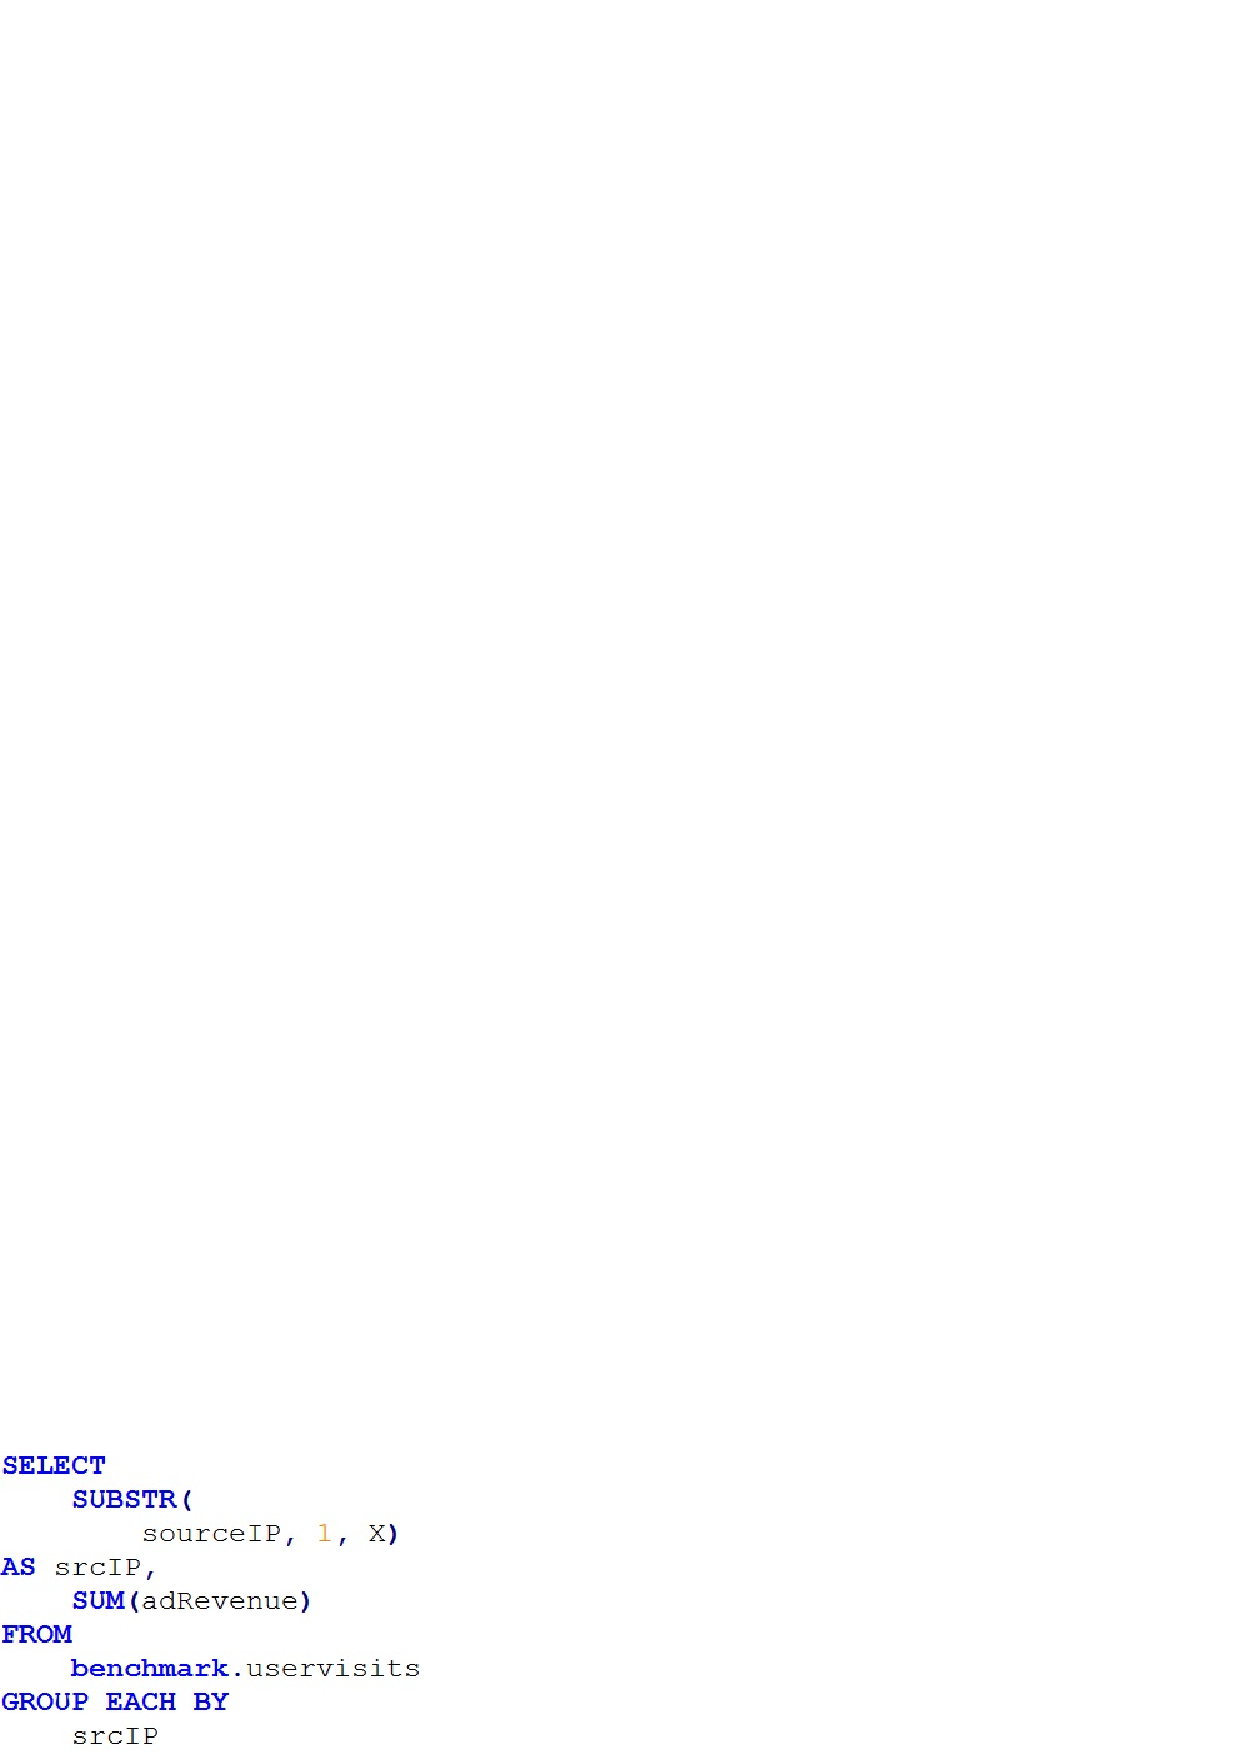
\includegraphics[width=\linewidth]{images/Query2}}
\caption{\cite{www-benchmarks-bigguery} Aggregation Query}
\label{fig:aggregationquery}
\end{figure}

This query has been fired using different values for 'X'. Query 2A
means X's value is 8, query 2B means X's value is 10 and 2C means X's
value is 12.

\item Join Query

Figure \ref{fig:joinquery} shows a join query between the rankings
table and uservisits table on some given condition.

\begin{figure}[htbp]
\centering
\fbox{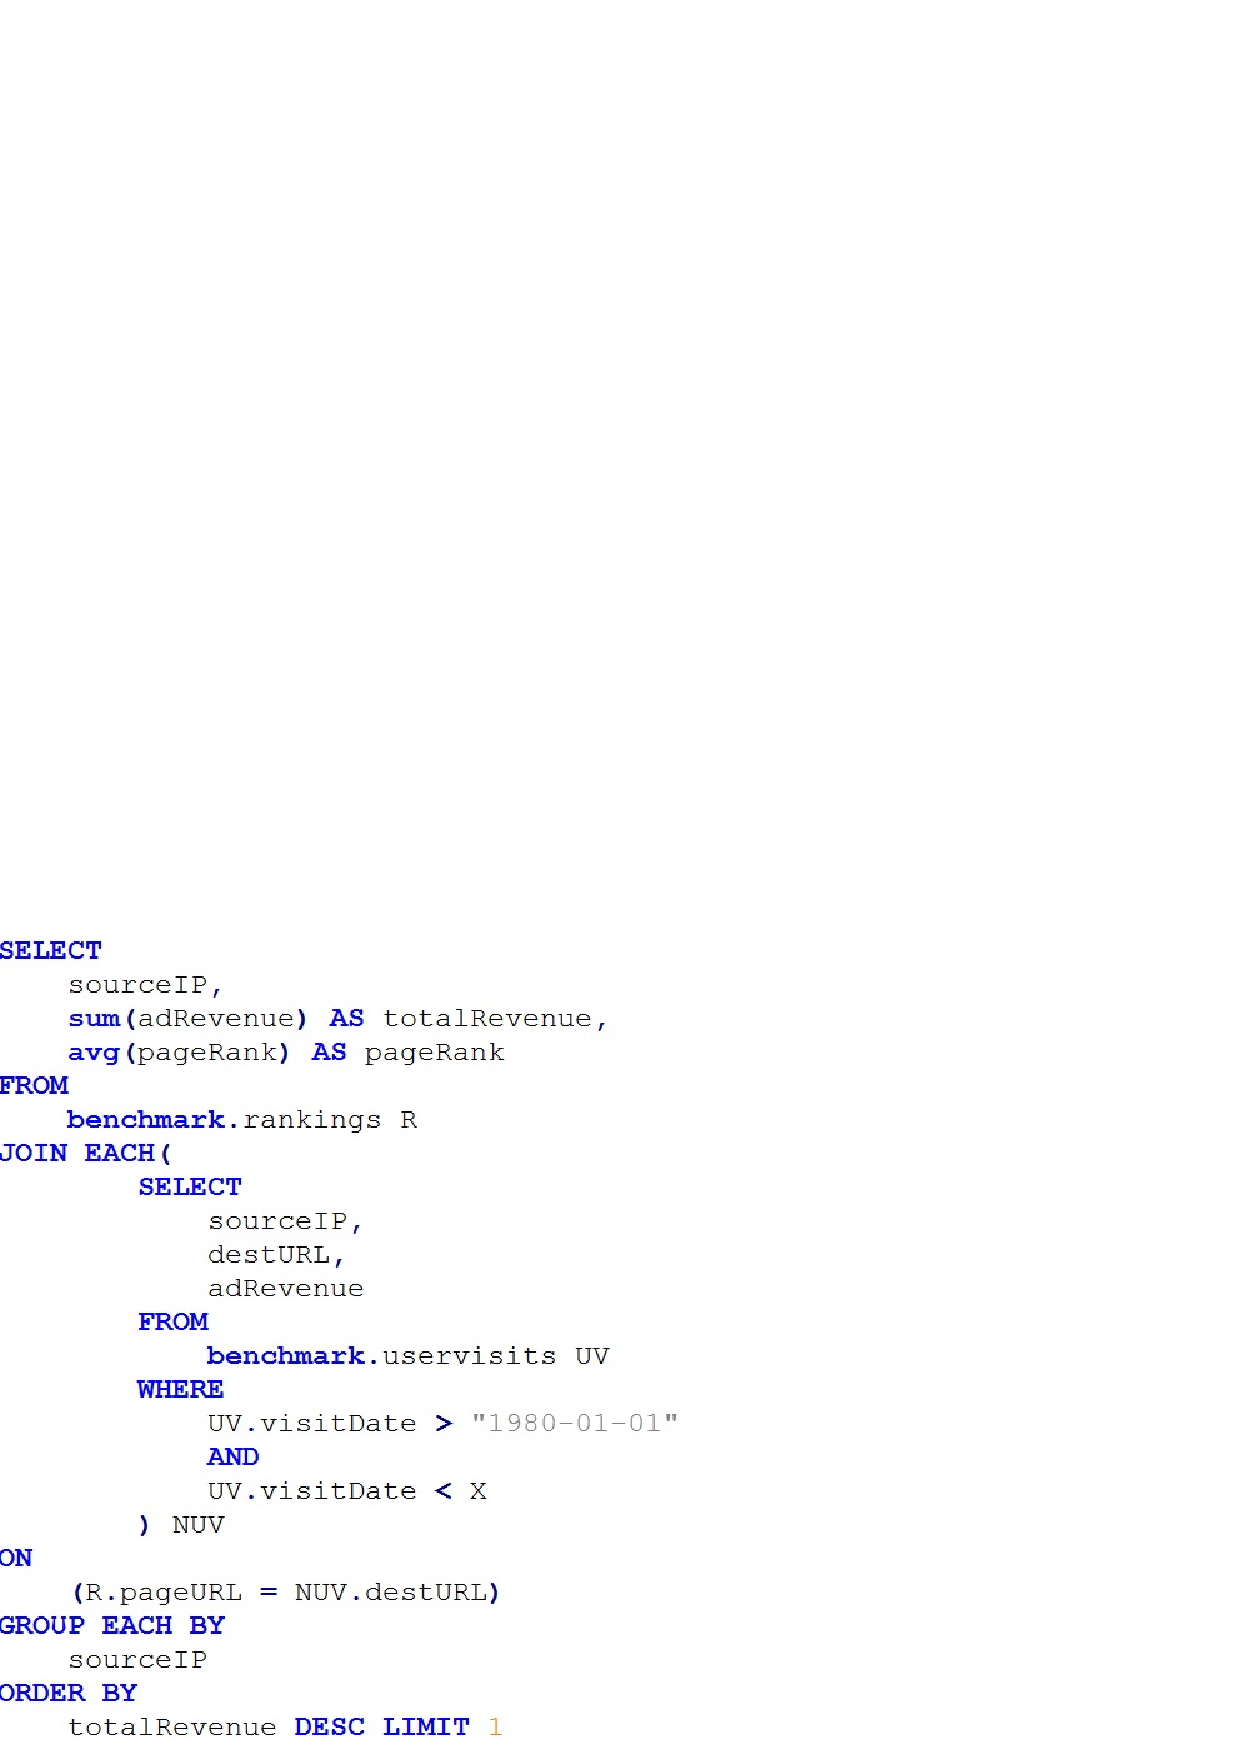
\includegraphics[width=\linewidth]{images/Query3}}
\caption{\cite{www-benchmarks-bigguery} Join Query}
\label{fig:joinquery}
\end{figure}

Like other queries earlier, this one also has different values for
'X'. Query 3A means X's value is ’1980-04-01’, query 3B means X is
’1983-01-01’ and 3C means X is ’2010-01-01’.

\end{enumerate}

\subsection{Comparison results}
\noindent
Figure \ref{fig:experiments} shows the results.

\begin{figure}[htbp]
\centering
\fbox{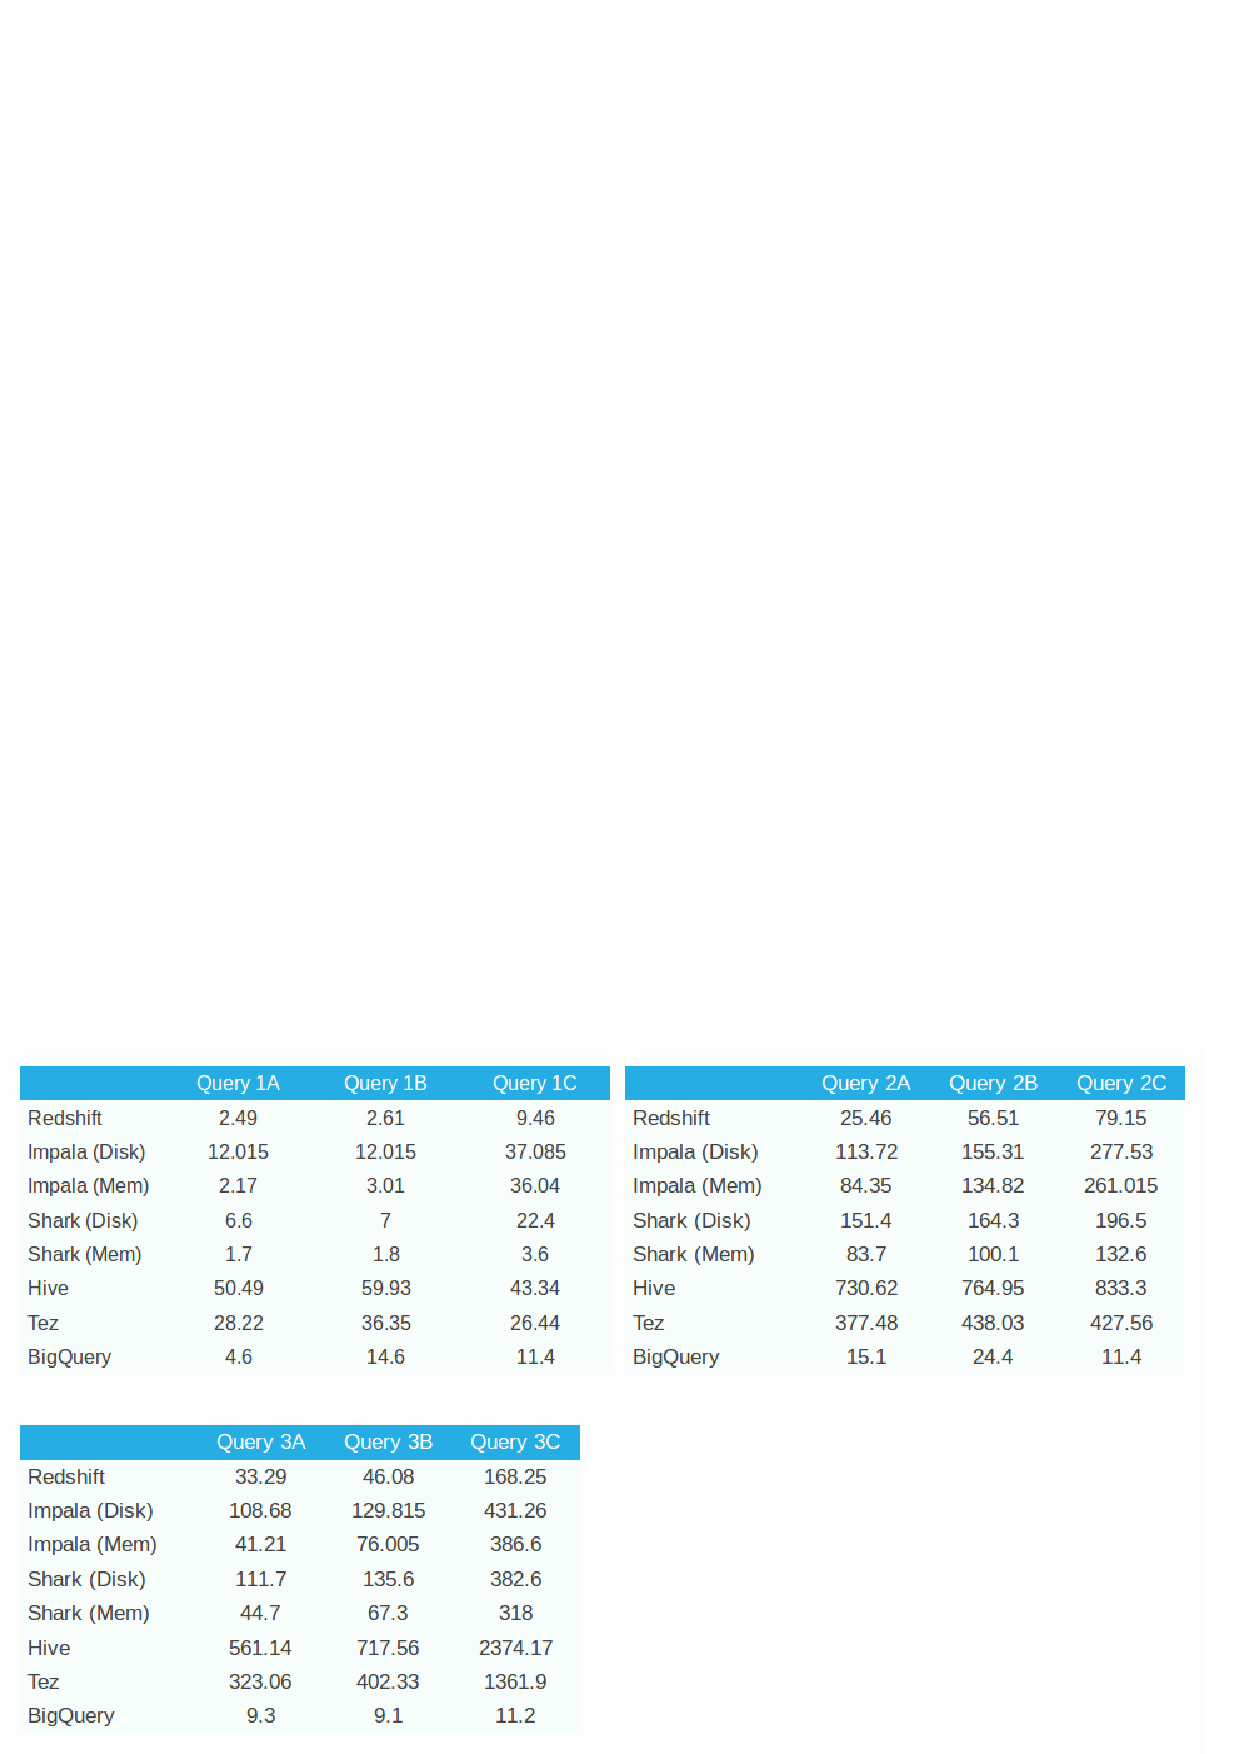
\includegraphics[width=\linewidth]{images/experiments}}
\caption{\cite{www-benchmarks-bigguery} Comparison of BigQuery with
  other storage platforms}
\label{fig:experiments}
\end{figure}

\noindent
In this comparison experiment, each query was executed atleast 10
times and the results which are displayed are the average values of
the response time in seconds. From \ref{fig:experiments}, it shows
that only in Query 1A, 1B and 1C BigQuery took more time than
Redshift, Impala (on memory) and Shark (on memory) but the results
related to query 2 and 3 are much better. For all the different values
of X in query 2 and 3 (A,B and C), BigQuery executed them faster than
other platforms. This shows that BigQuery can produce amazing results
when processing complex queries on large datasets. As the number of
processing records grew, BigQuery's response time was less as compared
to the other storage platforms.

\section{Use cases of BigQuery}
\subsection{Safari Books Online}
Safari Books Online\cite{www-usecase-safari} uses BigQuery to find
trends in customer purchase, manage its negative feedback related to
customer service, improve the sales team's effectiveness etc. They
chose BigQuery over other technologies because of its retrieval speed
by quering the datasets using a familiar SQL-like language, and the
lack of additional required maintenance.

\subsection{RedBus}
Online travel agency RedBus\cite{www-usecase-redbus} introduced
internet bus ticketing in India incorporating thousands of bus
schedules into a single booking operation. Using BigQuery, redBus was
able to manage the terabytes of booking and inventory data quickly and
at a lower cost than other big-data services. BigQuery also helped its
engineers fix glitches quickly, minimize lost sales and improve
customer service as well.

\section{Conclusion}
Google BigQuery is a cloud-based database service which enables to
process large data sets quickly. BigQuery allows to run SQL-like
queries against multiple gigabytes to terabytes of data in a matter of
seconds. It is suitable for ad-hoc OLAP/BI\cite{www-olap} queries that
require results as fast as possible. As a cloud-powered parallel query
database it provides extremely high full-scan query performance and
cost effectiveness compared to other traditional data warehouse
solutions and appliances.

\section*{Acknowledgements}

I would like to thank my professor Gregor von Laszewski and all the
associate instructors for their constant technical support.

% Bibliography

\bibliography{references}
 
\newpage

\appendix


\end{document}
